\documentclass[11pt, a4paper]{article}
\usepackage{graphicx}
\usepackage{amsmath}
\usepackage{listings}


\title{Assignment No 10: Spectra of Non-Periodic Signals}

\author{G Ch V Sairam , EE19B081}

\date{13-05-2021}
\begin{document}		
		
\maketitle
\section*{Introduction}
In this assignment, we explore the nature of DFTs of non-periodic signals, and the use of DFT in parameter estimation.These functions have a discontinuity when periodically extended. The discontinuity causes fourier components in frequencies other than the sinusoids frequency which decay as $1/\omega$, due to Gibbs phenomenon. 

\section*{Worked Example- Spectrum of $sin(\sqrt{2}t)$}
The given example of the spectrum of $sin(\sqrt{2}t)$ is discussed below:
Using the method followed for obtaining the DFT for periodic signals, the
following spectrum is obtained for $sin(\sqrt{2}t)$ :
 
\begin{figure}[!tbh]
\centering
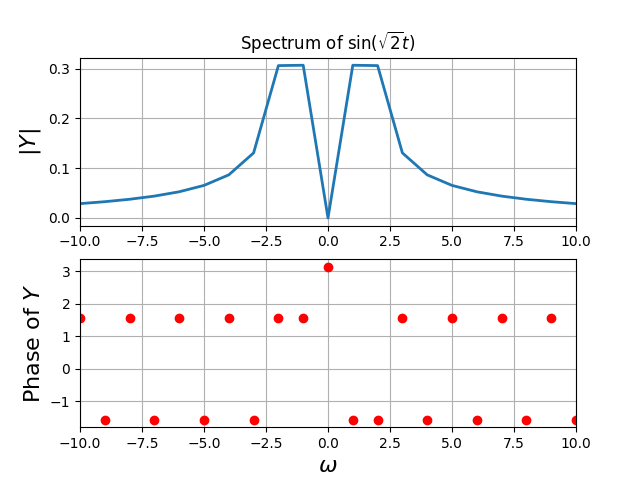
\includegraphics[scale=0.6]{assgn10_plot1.png} 
\label{fig1}
\end{figure} 

We expected two spikes, but what we got were two peaks each with two values and a gradually decaying magnitude. This is because, the DFT is trying to analyse the $2\pi$ periodic extension of the function in the interval [$-\pi$, $\pi$] . This function, having discontinuities, results in a slowly decaying frequency response and hence we do not obtain shark peaks at the expected frequencies. 
\newline
To understand where it went wrong, let's first plot the original function for which we want the DFT, over several time intervals.
 
\begin{figure}[!tbh]
\centering
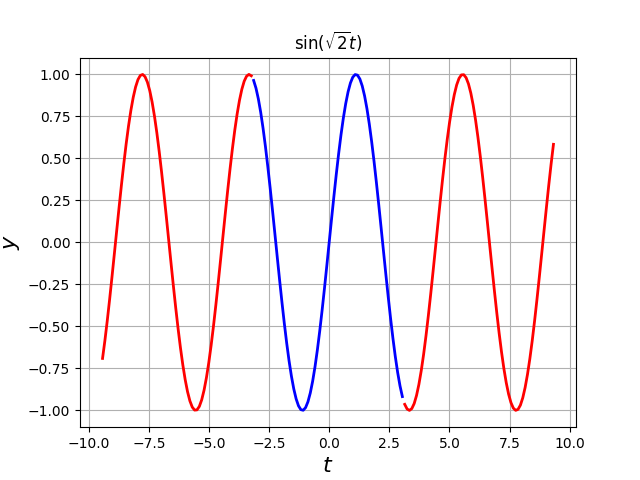
\includegraphics[scale=0.6]{assgn10_plot2.png} 
\label{fig2}
\end{figure} 

Quite clearly, even though $sin(\sqrt{2}t)$ is a periodic function, the portion between $-\pi$ and $\pi$ is not the part that can be replicated to generate the function. To find the exact function the DFT is tryning to analyse, let's just plot only the blue points. The graph is as below:

\begin{figure}[!tbh]
\centering
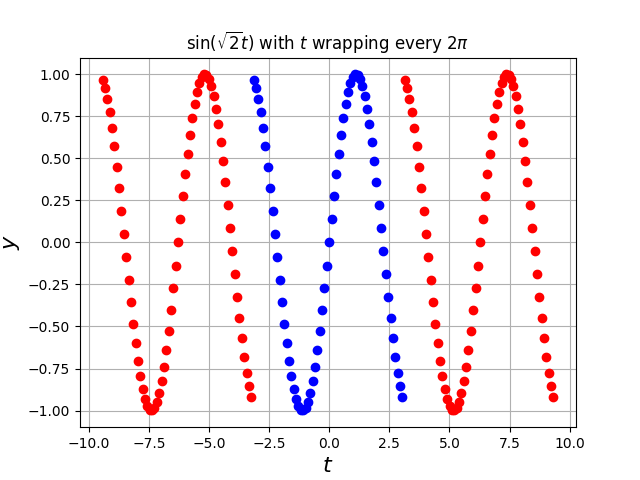
\includegraphics[scale=0.55]{assgn10_plot3.png} 
\label{fig3}
\end{figure} 

Clearly this function is not $sin(\sqrt{2}t)$, that is why the DFT is not what we expected.

\subsection*{Gibbs Phenomenon}
These discontinuities lead to non harmonic components in the FFT which decay as $1/\omega$ . This happens when the time samples are like the ramp. To verify this, we plot the spectrum of the periodic ramp below:

\begin{figure}[!tbh]
\centering
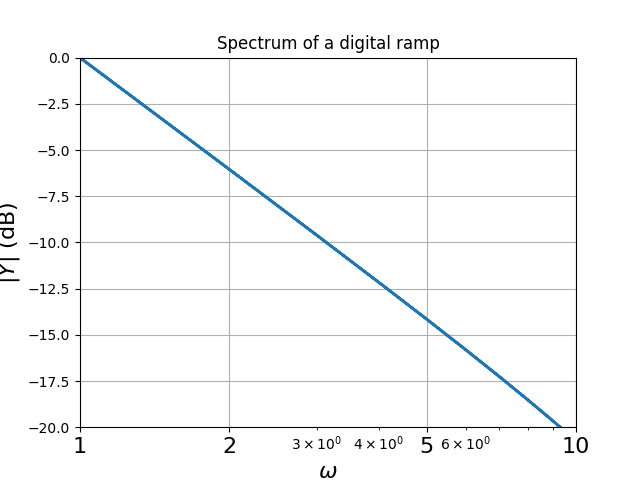
\includegraphics[scale=0.5]{assgn10_plot4.png} 
\label{fig4}
\end{figure} 

\subsection*{Hamming Window}
The fix for the above problem is windowing, where we multiply the function in the time domain with the Hamming window function :

\begin{equation*}
x[n] = 0.54 + 0.46cos(2\pi n/(N-1))
\end{equation*}

We now multiply our signal with the hamming window and periodically extend it. Note that the discontinuities nearly vanish

\begin{figure}[!tbh]
\centering
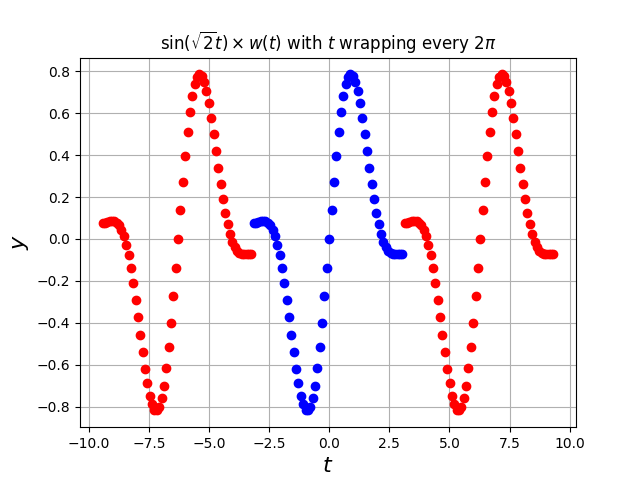
\includegraphics[scale=0.55]{assgn10_plot5.png} 
\label{fig5}
\end{figure} 

This happens because the hamming window removes discontinuities by attenuating the high frequency components causing the attenuities. But, the jump is still there, but it is much reduced.

When we take DFT of this sequence, we get:

\begin{figure}[!tbh]
\centering
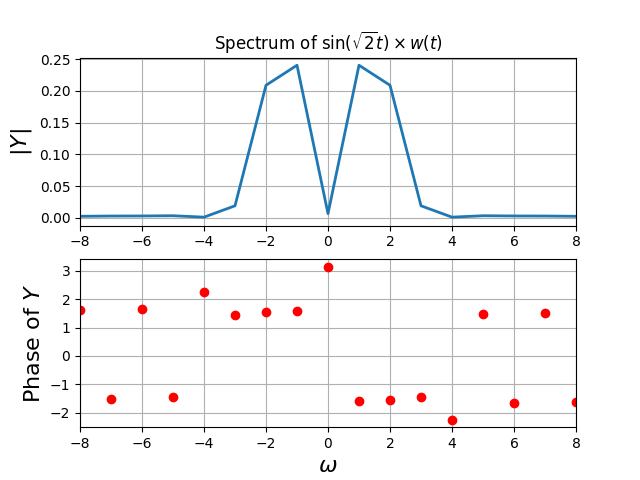
\includegraphics[scale=0.65]{assgn10_plot6.png} 
\label{fig6}
\end{figure} 

We still have a peak that is two samples wide. If we use more number of points, we will get better results.

\begin{figure}[!tbh]
\centering
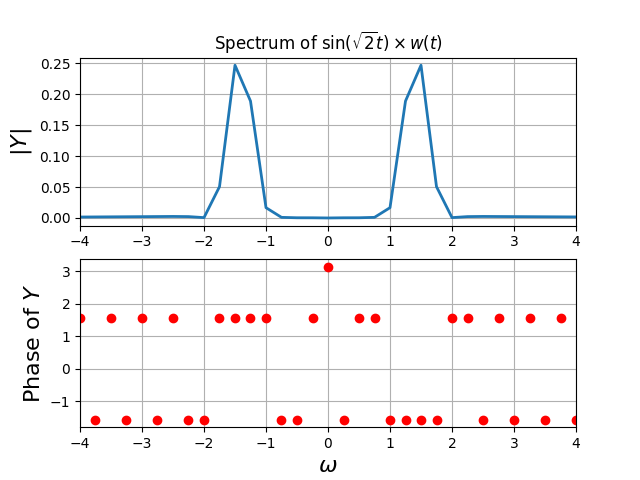
\includegraphics[scale=0.65]{assgn10_plot7.png} 
\label{fig7}
\end{figure} 

\section*{Assignment Questions}

The function to plot and return the DFT of an arbitrary function is given below.
\begin{verbatim}
def spectrum(lim,n,f,xlim1,title1,t_=True,t1=0,windowing=True,xlabel1 = r"$\omega$"
,ylabel1= r"Magnitude of Y", ylabel2 = r"Phase of Y",savename = "abc.png"):
		if t_:
			t=np.linspace(-lim,lim,n+1)[:-1]
		else:
			t=t1
		dt=t[1]-t[0]
		fmax=1/dt
		y = f(t)
		if (windowing):
			m=np.arange(n)
			wnd=np.fft.fftshift(0.54+0.46*np.cos(2*pi*m/n))
			y = y*wnd
		y[0]=0
		y=np.fft.fftshift(y)
		Y=np.fft.fftshift(np.fft.fft(y))/float(n)
		w=np.linspace(-pi*fmax,pi*fmax,n+1)[:-1]
		
		mag = np.abs(Y)
		phi = np.angle(Y)
		plt.figure()
		plt.subplot(2,1,1)
		plt.plot(w,mag,lw=2)
		plt.xlim([-xlim1,xlim1])
		plt.ylabel(ylabel1,size=16)
		plt.title(title1)
		plt.grid(True)
		plt.subplot(2,1,2)
		phi[np.where(mag<3e-3)] = 0
		plt.plot(w,phi,'ro',lw=2)
		plt.xlim([-xlim1,xlim1])
		plt.ylabel(ylabel2,size=16)
		plt.xlabel(xlabel1,size=16)
		plt.grid(True)
		plt.savefig(savename)
		plt.show()
		return w,Y
\end{verbatim}

\subsection*{Spectrum of $cos^3(0.86t)$}
The Spectrum of $cos^3(w_ot)$ for $w_o$ = 0.86 without windowing is as follows:

\begin{figure}[!tbh]
\centering
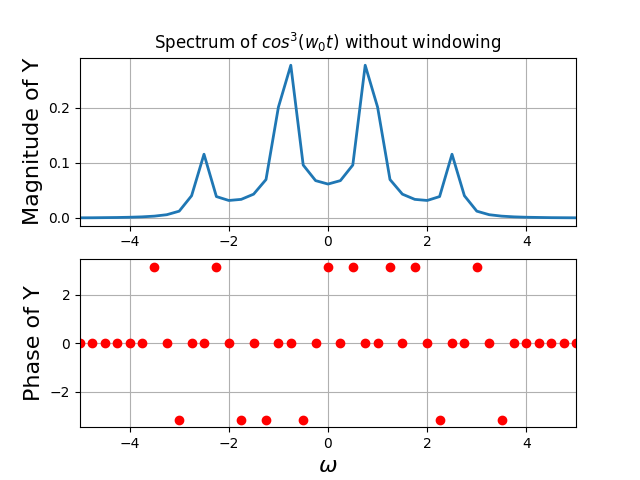
\includegraphics[scale=0.72]{assgn10_plot8.png} 
\label{fig8}
\end{figure} 

The Spectrum after windowing has a narrower peak :
\begin{figure}[!tbh]
\centering
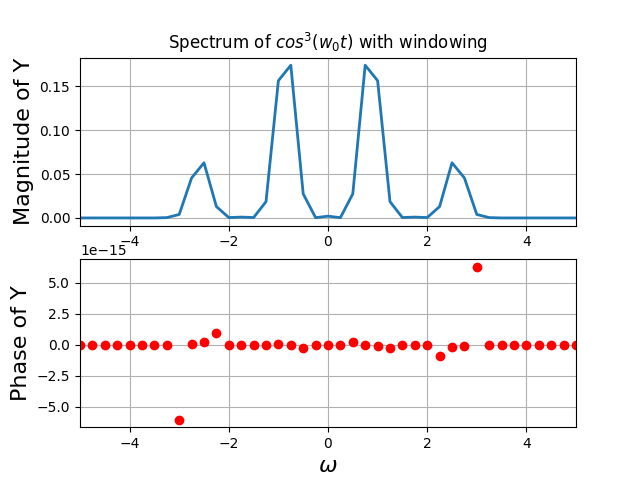
\includegraphics[scale=0.72]{assgn10_plot9.png} 
\label{fig9}
\end{figure} 

In the plot without windowing, we notice that a lot of the energy is stored in the frequencies that are not a part of the signal. After windowing, these frequencies are attenuated and hence the peaks are sharper in the windowed function. It is still not an impulse because the convolution with the Fourier transform of the windowed function smears out the peak.

\subsection*{Estimation of $\omega$ and $\delta$ in DFT}
We need to estimate $\omega$ and $\delta$ for a signal cos($\omega$t+$\delta$) for 128 samples between [-$\pi$, $\pi$). We estimate omega using a weighted average. We have to extract the digital spectrum of the signal and find the two peaks at $\omega$, and estimate $\omega$ and $\delta$.

The function to do this is given below:
\begin{verbatim}

	ii = np.where(w >= 0)
	sol_w = np.sum(w[ii][:5]*np.absolute(Y)[ii][:5])/np.sum(np.absolute(Y)[ii][:5])
	kk = np.argmax(np.absolute(Y[ii]))
	sol_delta = np.angle(Y[ii])[kk]
	print ("Estimated omega = ", sol_w)
	print ("Estimated delta=",sol_delta)#weighted average for first 2 points

\end{verbatim}

The digital spectrum for the given signal is:

\begin{figure}[!tbh]
\centering
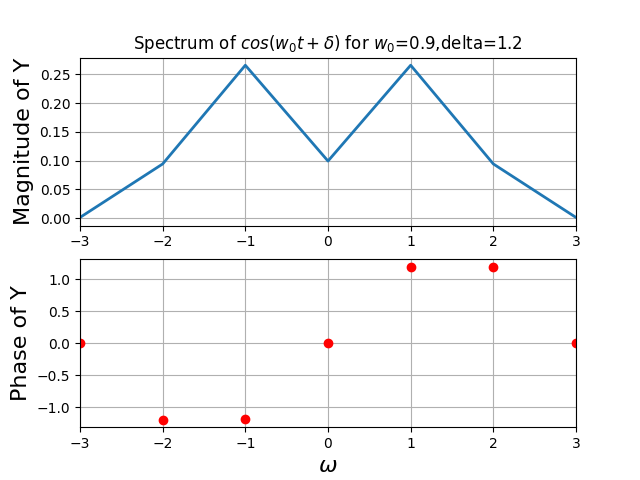
\includegraphics[scale=0.7]{assgn10_plot10.png} 
\label{fig10}
\end{figure} 

Estimating the values of $\omega$ and $\delta$, we get the output:
\begin{verbatim}
Actual omega= 0.9
Actual delta= 1.2 

Estimated omega =  1.0002825327219154
Estimated delta= 1.194423616699812
\end{verbatim}

\subsection*{Estimation in the case of noisy data}
We follow a process similar as above. The only change is the function being used.
\newline
The digital spectrum for the noisy signal:
\begin{figure}[!tbh]
\centering
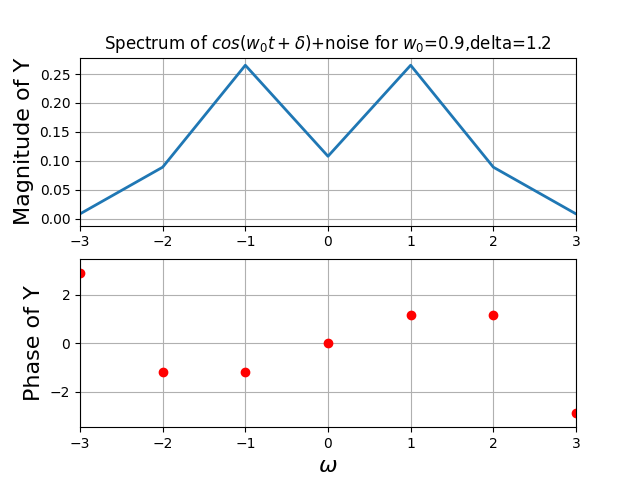
\includegraphics[scale=0.7]{assgn10_plot11.png} 
\label{fig11}
\end{figure}

Estimating the output, we get:
\begin{verbatim}
After adding white gaussian noise: 

Estimated omega =  1.0156459531567994
Estimated delta= 1.2084321129087388
\end{verbatim}

\subsection*{DFT of a chirped signal}
We analyze a chirp signal which is an FM signal where frequency is directly proportional to time. The chirp signal we shall consider is given by:
\begin{equation*}
 f(t)=cos(16t(1.5+t/2\pi))
\end{equation*}
The chirped signal is a signal of varying frequency, with frequency increasing from 16 to 32 radians per second as we move from -$\pi$ to $\pi$ .

The spectrum of this signal without a hamming window is given by:
\begin{figure}[!tbh]
\centering
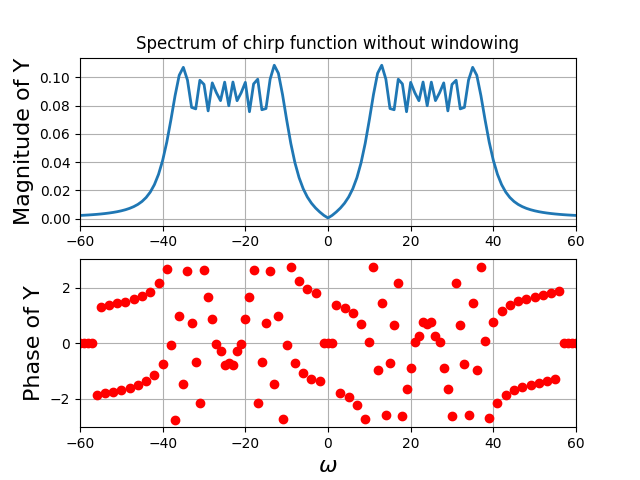
\includegraphics[scale=0.7]{assgn10_plot12.png} 
\label{fig12}
\end{figure}

We note that the frequency response is spread between 5-50 rad/s. A large section of this range apears due to Gibbs phenomenon. On windowing, only frequencies between 16 and 32 rad/s remain.

\begin{figure}[!tbh]
\centering
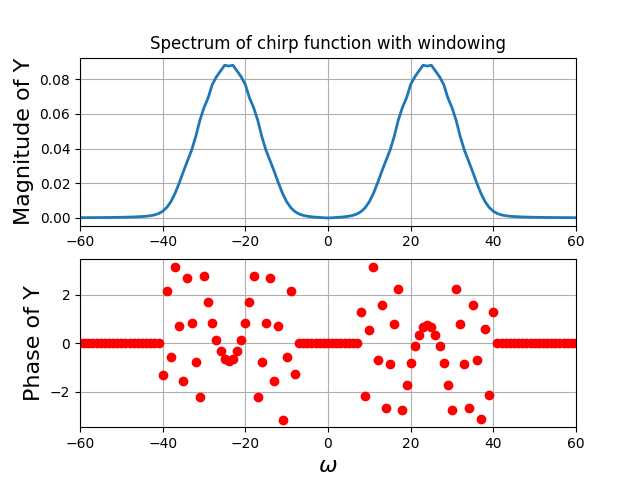
\includegraphics[scale=0.7]{assgn10_plot13.png} 
\label{fig13}
\end{figure}

\newpage
\subsection*{Time-Frequency plot for the chirped signal}
On breaking the 1024 length vector into 16 pieces, each 64 samples wide, we can analyse the DFT in how it evolves over time. We plot a “time- frequency” plot, where we get localized DFTs and show how the spectrum evolves in time.

The time-frequency plot of the Chirped signal without a hamming window:
\begin{figure}[!tbh]
\centering
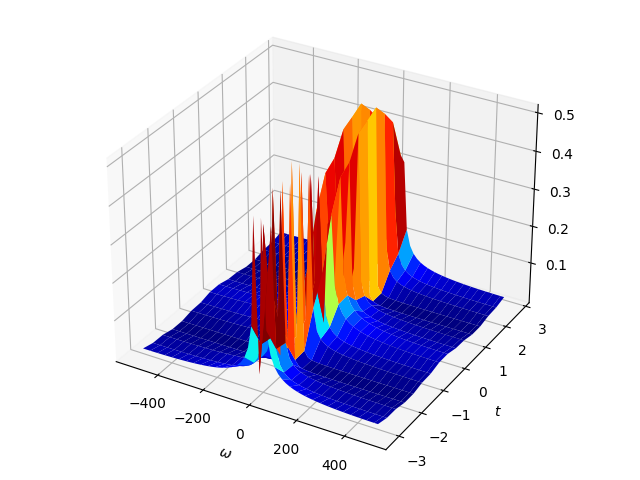
\includegraphics[scale=0.63]{assgn10_plot14.png} 
\label{fig14}
\end{figure}

After windowing, the plot changes to:
\begin{figure}[!tbh]
\centering
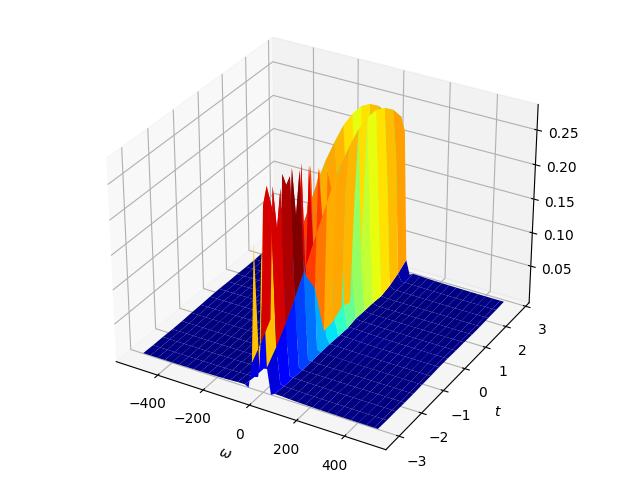
\includegraphics[scale=0.63]{assgn10_plot15.png} 
\label{fig15}
\end{figure}

\section*{Conclusion}
The DFT was obtained using a 2$\pi$ periodic extension of the signal, and thus the spectrum was found to be erroneous for a non periodic function. The spectrum was rectified by the using a windowing technique, by employing the Hamming window. Given a vector of cosine values in the a time interval, the frequency and phase were estimated from the DFT spectrum, by using the expectation value of the frequency and a parameter grid search for optimum values. The DFT of a chirped signal was analysed and its time-frequency plot showed the gradual variation of peak frequency of the spectrum with time.

\end{document}